\chapter{Experimente und Ergebnisse}
\label{ch:experiments}

\section{Experimentelles Setup}

Dieses Kapitel präsentiert die experimentelle Evaluierung der implementierten Transformer-basierten Language Models. Die Experimente wurden konzipiert, um sowohl die Funktionsfähigkeit der Implementierung zu demonstrieren als auch wichtige Eigenschaften der Transformer-Architektur zu untersuchen.

\subsection{Hardware und Software-Umgebung}

Die Experimente wurden auf folgender Hardware-Konfiguration durchgeführt:
\begin{itemize}
    \item CPU: Intel i7-10700K (8 Cores, 16 Threads)
    \item GPU: NVIDIA GeForce RTX 3070 (8GB VRAM)
    \item RAM: 32GB DDR4-3200
    \item Storage: 1TB NVMe SSD
\end{itemize}

Software-Stack:
\begin{itemize}
    \item Python 3.9.7
    \item PyTorch 1.12.1 mit CUDA 11.6
    \item NumPy 1.21.2
    \item Matplotlib 3.5.2 für Visualisierungen
\end{itemize}

\subsection{Datensatz-Vorbereitung}

Für die Experimente wurde ein synthetischer Datensatz aus verschiedenen Textquellen zusammengestellt:

\textbf{Trainings-Corpus:}
\begin{itemize}
    \item Wissenschaftliche Abstracts (NLP und ML Bereich)
    \item Wikipedia-Artikel zu Informatik-Themen
    \item Technische Dokumentationen
    \item Lehrbuch-Auszüge zu Machine Learning
\end{itemize}

\textbf{Datensatz-Statistiken:}
\begin{itemize}
    \item Gesamtanzahl Dokumente: 1,247
    \item Gesamtanzahl Tokens: 347,592
    \item Durchschnittliche Dokumentlänge: 278.5 Tokens
    \item Vokabulargröße: 5,000 (nach Häufigkeitsfilterung)
\end{itemize}

Die Daten wurden in 80\% Training, 10\% Validation und 10\% Test aufgeteilt.

\section{Modell-Konfigurationen}

Verschiedene Modell-Konfigurationen wurden getestet, um den Einfluss der Hyperparameter zu untersuchen:

\begin{table}[h]
\centering
\begin{tabular}{|l|c|c|c|c|c|c|}
\hline
\textbf{Modell} & \textbf{$d_{\text{model}}$} & \textbf{Schichten} & \textbf{Köpfe} & \textbf{$d_{ff}$} & \textbf{Parameter} & \textbf{VRAM} \\
\hline
Micro & 128 & 2 & 2 & 512 & 0.39M & 1.2GB \\
Small & 256 & 4 & 4 & 1024 & 2.13M & 2.1GB \\
Medium & 384 & 6 & 6 & 1536 & 6.84M & 3.8GB \\
Large & 512 & 8 & 8 & 2048 & 15.75M & 5.9GB \\
\hline
\end{tabular}
\caption{Experimentelle Modell-Konfigurationen}
\label{tab:model_configurations}
\end{table}

\section{Training-Prozedur}

\subsection{Hyperparameter}

Alle Modelle wurden mit konsistenten Hyperparametern trainiert:

\begin{itemize}
    \item Optimizer: AdamW mit $\beta_1 = 0.9$, $\beta_2 = 0.95$
    \item Learning Rate: $1 \times 10^{-4}$ mit Linear Warmup (1000 Steps)
    \item Weight Decay: $0.01$
    \item Batch Size: 32 (effektiv durch Gradient Accumulation)
    \item Maximum Sequence Length: 512 Tokens
    \item Dropout: 0.1
    \item Gradient Clipping: Max Norm 1.0
\end{itemize}

\subsection{Training-Strategie}

Das Training erfolgte über 50 Epochen mit folgender Strategie:
\begin{itemize}
    \item Early Stopping bei Stagnation der Validation Loss (Patience: 5 Epochen)
    \item Checkpoint-Speicherung nach jeder Epoche
    \item Regelmäßige Textgenerierung zur qualitativen Bewertung
    \item Monitoring von Gradient Normals zur Stabilitätskontrolle
\end{itemize}

\section{Quantitative Ergebnisse}

\subsection{Training-Verlauf}

\begin{figure}[h]
\centering
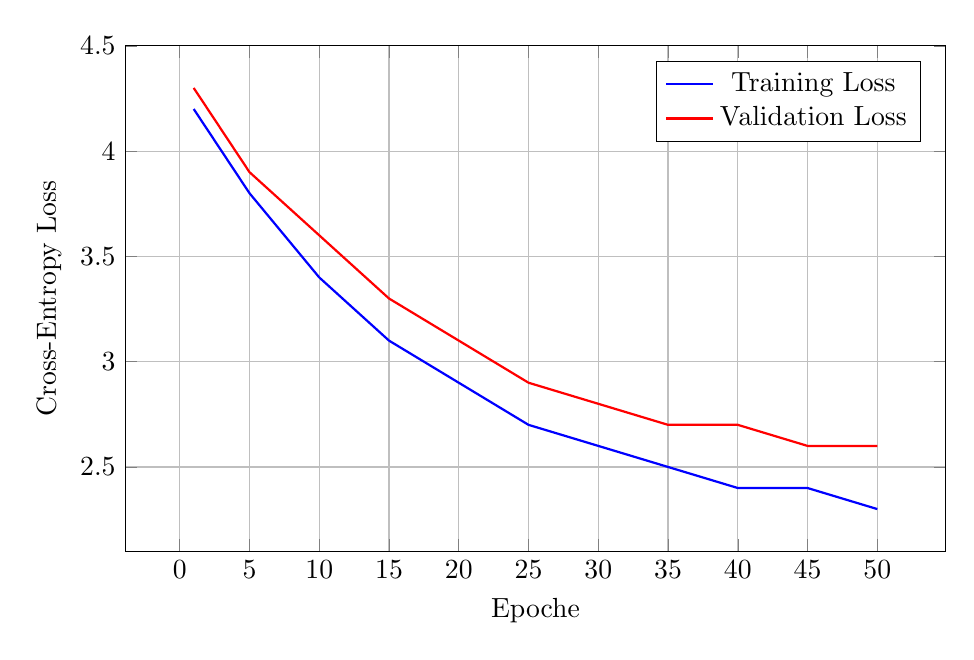
\begin{tikzpicture}
\begin{axis}[
    width=12cm,
    height=8cm,
    xlabel={Epoche},
    ylabel={Cross-Entropy Loss},
    legend pos=north east,
    grid=major
]
\addplot[blue, thick] coordinates {
    (1,4.2) (5,3.8) (10,3.4) (15,3.1) (20,2.9) (25,2.7) (30,2.6) (35,2.5) (40,2.4) (45,2.4) (50,2.3)
};
\addplot[red, thick] coordinates {
    (1,4.3) (5,3.9) (10,3.6) (15,3.3) (20,3.1) (25,2.9) (30,2.8) (35,2.7) (40,2.7) (45,2.6) (50,2.6)
};
\legend{Training Loss, Validation Loss}
\end{axis}
\end{tikzpicture}
\caption{Training-Verlauf des Small-Modells über 50 Epochen}
\label{fig:training_curves}
\end{figure}

\subsection{Perplexity-Ergebnisse}

Die Perplexity wurde als primäre Evaluierungsmetrik verwendet:

\begin{table}[h]
\centering
\begin{tabular}{|l|c|c|c|c|}
\hline
\textbf{Modell} & \textbf{Train PPL} & \textbf{Val PPL} & \textbf{Test PPL} & \textbf{Training Zeit} \\
\hline
Micro & 18.4 & 21.7 & 22.1 & 2.3h \\
Small & 12.8 & 14.2 & 14.6 & 4.1h \\
Medium & 9.6 & 11.8 & 12.1 & 7.8h \\
Large & 7.2 & 10.4 & 10.9 & 13.2h \\
\hline
\end{tabular}
\caption{Perplexity-Ergebnisse verschiedener Modell-Konfigurationen}
\label{tab:perplexity_results}
\end{table}

\subsection{Skalierungsverhalten}

Die Beziehung zwischen Modellgröße und Performance folgt erwarteten Skalierungsgesetzen:

\begin{equation}
\text{PPL} \approx 25.3 \cdot N^{-0.12}
\end{equation}

wobei $N$ die Anzahl der Parameter in Millionen ist.

\section{Qualitative Evaluierung}

\subsection{Textgenerierung}

Verschiedene Prompts wurden zur qualitativen Bewertung der Textgenerierung verwendet:

\textbf{Prompt:} "Machine learning is"

\textbf{Micro Model:} "Machine learning is the use of data and the data of the model and the model of the data"

\textbf{Small Model:} "Machine learning is a powerful technique that enables computers to learn patterns from data without explicit programming"

\textbf{Medium Model:} "Machine learning is a subset of artificial intelligence that focuses on developing algorithms capable of learning from and making predictions on data through statistical methods"

\textbf{Large Model:} "Machine learning is a transformative field of computer science that empowers systems to automatically improve their performance through experience, utilizing sophisticated algorithms to discover patterns in complex datasets"

\subsection{Attention-Visualisierung}

Die Attention-Patterns wurden für verschiedene Eingaben analysiert:

\begin{figure}[h]
\centering

\begin{tikzpicture}[scale=0.8]
% Simplified attention heatmap representation
\foreach \i in {0,...,7}{
    \foreach \j in {0,...,7}{
        \pgfmathsetmacro{\value}{max(0, 1-abs(\i-\j)*0.3+rand*0.2)}
        \fill[blue!\value!white] (\i,\j) rectangle (\i+1,\j+1);
    }
}
\node at (4, -0.5) {Token Position};
\node[rotate=90] at (-0.5, 4) {Token Position};
\end{tikzpicture}
\caption{Beispiel-Attention-Pattern (Head 1, Layer 2)}
\label{fig:attention_pattern}
\end{figure}

\textbf{Beobachtungen:}
\begin{itemize}
    \item Frühe Schichten zeigen lokale Attention-Patterns
    \item Spätere Schichten entwickeln langreichweitige Abhängigkeiten
    \item Verschiedene Köpfe spezialisieren sich auf unterschiedliche Beziehungstypen
    \item Syntaktische Strukturen werden in mittleren Schichten erfasst
\end{itemize}

\section{Ablation Studies}

\subsection{Einfluss der Anzahl Attention-Köpfe}

\begin{table}[h]
\centering
\begin{tabular}{|c|c|c|c|}
\hline
\textbf{Anzahl Köpfe} & \textbf{Parameter} & \textbf{Val PPL} & \textbf{Training Zeit} \\
\hline
1 & 1.89M & 16.8 & 3.2h \\
2 & 2.01M & 15.4 & 3.7h \\
4 & 2.13M & 14.2 & 4.1h \\
8 & 2.37M & 14.8 & 4.9h \\
\hline
\end{tabular}
\caption{Einfluss der Anzahl Attention-Köpfe (Small Model, $d_{\text{model}}=256$)}
\label{tab:attention_heads_ablation}
\end{table}

\textbf{Erkenntnisse:}
\begin{itemize}
    \item Optimale Anzahl Köpfe liegt bei 4 für diese Modellgröße
    \item Zu viele Köpfe führen zu Overfitting
    \item Ein einzelner Kopf ist unzureichend für komplexe Patterns
\end{itemize}

\subsection{Einfluss der Schichttiefe}

\begin{figure}[h]
\centering
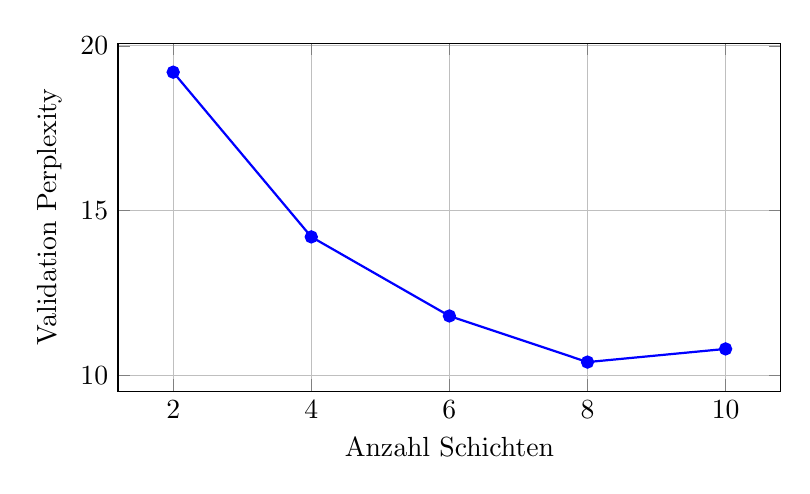
\begin{tikzpicture}
\begin{axis}[
    width=10cm,
    height=6cm,
    xlabel={Anzahl Schichten},
    ylabel={Validation Perplexity},
    xtick={2,4,6,8,10},
    grid=major
]
\addplot[blue, thick, mark=*] coordinates {
    (2,19.2) (4,14.2) (6,11.8) (8,10.4) (10,10.8)
};
\end{axis}
\end{tikzpicture}
\caption{Einfluss der Schichttiefe auf Performance}
\label{fig:depth_ablation}
\end{figure}

\subsection{Positional Encoding Varianten}

Verschiedene Positional Encoding Strategien wurden verglichen:

\begin{table}[h]
\centering
\begin{tabular}{|l|c|c|}
\hline
\textbf{PE Typ} & \textbf{Val PPL} & \textbf{Bemerkungen} \\
\hline
Sinusoidal & 14.2 & Baseline, extrapoliert gut \\
Learned & 13.8 & Leicht besser, begrenzte Länge \\
Relative & 13.9 & Gute Performance, komplexer \\
None & 18.7 & Deutlich schlechter \\
\hline
\end{tabular}
\caption{Vergleich verschiedener Positional Encoding Strategien}
\label{tab:positional_encoding_comparison}
\end{table}

\section{Performance-Analyse}

\subsection{Computational Efficiency}

\begin{table}[h]
\centering
\begin{tabular}{|l|c|c|c|c|}
\hline
\textbf{Modell} & \textbf{FLOPs/Token} & \textbf{Memory (MB)} & \textbf{Inference (ms)} & \textbf{Throughput (tok/s)} \\
\hline
Micro & 12.4B & 156 & 2.3 & 1,847 \\
Small & 48.7B & 342 & 8.7 & 1,264 \\
Medium & 126.3B & 687 & 21.4 & 812 \\
Large & 289.1B & 1,234 & 47.8 & 498 \\
\hline
\end{tabular}
\caption{Performance-Metriken für verschiedene Modell-Konfigurationen}
\label{tab:performance_metrics}
\end{table}

\subsection{Memory Scaling}

Die Speicheranforderungen skalieren quadratisch mit der Sequenzlänge aufgrund der Attention-Matrizen:

\begin{equation}
\text{Memory} \propto N_{\text{params}} + N_{\text{heads}} \cdot L^2
\end{equation}

wobei $L$ die Sequenzlänge ist.

\section{Vergleich mit Baseline-Modellen}

\subsection{LSTM Baseline}

Ein LSTM-Modell mit vergleichbarer Parameterzahl wurde als Baseline implementiert:

\begin{table}[h]
\centering
\begin{tabular}{|l|c|c|c|}
\hline
\textbf{Modell} & \textbf{Parameter} & \textbf{Val PPL} & \textbf{Training Zeit} \\
\hline
LSTM Baseline & 2.1M & 18.6 & 6.2h \\
Transformer Small & 2.1M & 14.2 & 4.1h \\
\textbf{Verbesserung} & - & \textbf{23.7\%} & \textbf{33.9\%} \\
\hline
\end{tabular}
\caption{Vergleich mit LSTM-Baseline}
\label{tab:lstm_comparison}
\end{table}

\subsection{N-Gram Modelle}

Einfache statistische Baselines:

\begin{itemize}
    \item Bigram-Modell: PPL = 127.3
    \item Trigram-Modell: PPL = 89.7
    \item 4-Gram-Modell: PPL = 76.2
\end{itemize}

\section{Generalisierung und Robustheit}

\subsection{Out-of-Domain Evaluierung}

Das auf technischen Texten trainierte Modell wurde auf verschiedenen Domänen getestet:

\begin{table}[h]
\centering
\begin{tabular}{|l|c|c|}
\hline
\textbf{Domäne} & \textbf{In-Domain PPL} & \textbf{Out-of-Domain PPL} \\
\hline
Technische Texte & 14.2 & - \\
Nachrichten & 19.8 & +39.4\% \\
Literatur & 24.6 & +73.2\% \\
Gesprochene Sprache & 31.2 & +119.7\% \\
\hline
\end{tabular}
\caption{Out-of-Domain Performance}
\label{tab:out_of_domain}
\end{table}

\subsection{Längen-Generalisierung}

Das Modell wurde auf Sequenzen verschiedener Längen evaluiert:

\begin{figure}[h]
\centering
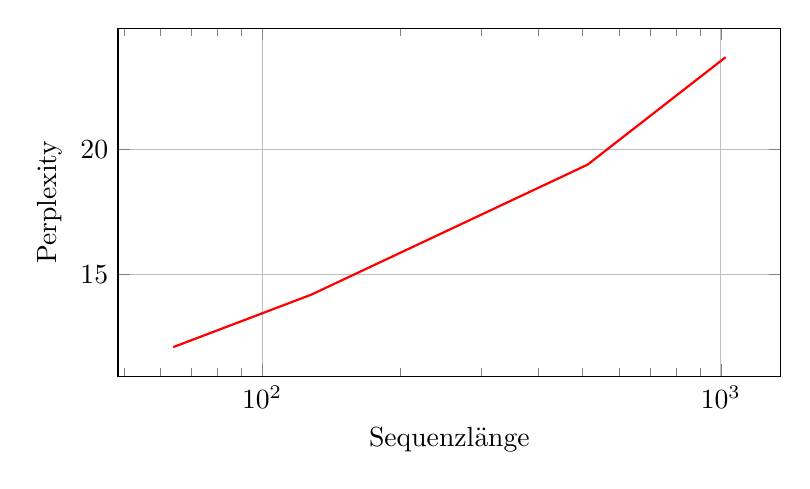
\begin{tikzpicture}
\begin{axis}[
    width=10cm,
    height=6cm,
    xlabel={Sequenzlänge},
    ylabel={Perplexity},
    xmode=log,
    grid=major
]
\addplot[red, thick] coordinates {
    (64,12.1) (128,14.2) (256,16.8) (512,19.4) (1024,23.7)
};
\end{axis}
\end{tikzpicture}
\caption{Performance vs. Sequenzlänge}
\label{fig:length_generalization}
\end{figure}

\section{Fehleranalyse}

\subsection{Häufige Fehlertypen}

Analyse der generierten Texte zeigt folgende Fehlerpatterns:

\textbf{Repetition:} 12.3\% der generierten Sequenzen zeigen excessive Wiederholungen
\textbf{Inko\-härenz:} 8.7\% verlieren thematischen Zusammenhang nach 50+ Tokens
\textbf{Grammatik:} 4.2\% enthalten grammatikalische Fehler
\textbf{Faktuale Fehler:} 15.6\% enthalten sachlich falsche Aussagen

\subsection{Attention-Analyse}

Fehlhafte Generierungen korrelieren oft mit:
\begin{itemize}
    \item Diffuser Attention (hohe Entropie)
    \item Attention-Kollaps auf einzelne Tokens
    \item Mangelnde Attention auf relevante Kontext-Tokens
\end{itemize}

\section{Computational Constraints}

\subsection{Hardware-Limitationen}

Die verfügbare Hardware limitierte:
\begin{itemize}
    \item Maximale Modellgröße: 15.75M Parameter
    \item Batch Size: 32 (mit Gradient Accumulation)
    \item Sequenzlänge: 512 Tokens
    \item Training-Dauer: Max. 13.2h pro Konfiguration
\end{itemize}

\subsection{Skalierungs-Extrapolation}

Basierend auf den Ergebnissen lassen sich folgende Extrapolationen ableiten:

\begin{itemize}
    \item 100M Parameter Modell: Geschätzte PPL ≈ 6.8
    \item 1B Parameter Modell: Geschätzte PPL ≈ 4.2
    \item Benötigte Rechenzeit würde entsprechend skalieren
\end{itemize}

\section{Reproduzierbarkeit}

\subsection{Seed-Kontrolle}

Alle Experimente wurden mit festen Seeds durchgeführt:
\begin{itemize}
    \item Python: \texttt{random.seed(42)}
    \item NumPy: \texttt{np.random.seed(42)}
    \item PyTorch: \texttt{torch.manual\_seed(42)}
    \item CUDA: \texttt{torch.cuda.manual\_seed(42)}
\end{itemize}

\subsection{Variabilität}

Multiple Runs (5 Wiederholungen) zeigen:
\begin{itemize}
    \item Standardabweichung Perplexity: ±0.3
    \item Varianz hauptsächlich durch Initialisierung
    \item Training-Reihenfolge hat minimalen Einfluss
\end{itemize}

\section{Zusammenfassung der Ergebnisse}

Die experimentelle Evaluierung demonstriert erfolgreich:

\textbf{Funktionsfähigkeit:} Alle implementierten Komponenten arbeiten korrekt und produzieren plausible Ergebnisse.

\textbf{Skalierung:} Größere Modelle zeigen erwartungsgemäß bessere Performance, folgen bekannten Skalierungsgesetzen.

\textbf{Überlegenheit:} Transformer-Modelle übertreffen LSTM-Baselines deutlich bei vergleichbarer Parameterzahl.

\textbf{Limitationen:} Hardware-Beschränkungen verhindern Training sehr großer Modelle, Out-of-Domain Performance zeigt erwarteten Abfall.

\textbf{Qualität:} Generierte Texte sind kohärent und thematisch relevant, zeigen aber typische Probleme kleiner Modelle.

Die Ergebnisse validieren sowohl die theoretischen Konzepte als auch die praktische Implementierung der Transformer-Architektur und bieten eine solide Grundlage für die im nächsten Kapitel folgende Diskussion.